\section{AL\_\-Day  Class Reference}
\label{classAL__Day}\index{AL_Day@{AL\_\-Day}}
{\tt \#include $<$dil2al.hh$>$}

Inheritance diagram for AL\_\-Day::\begin{figure}[H]
\begin{center}
\leavevmode
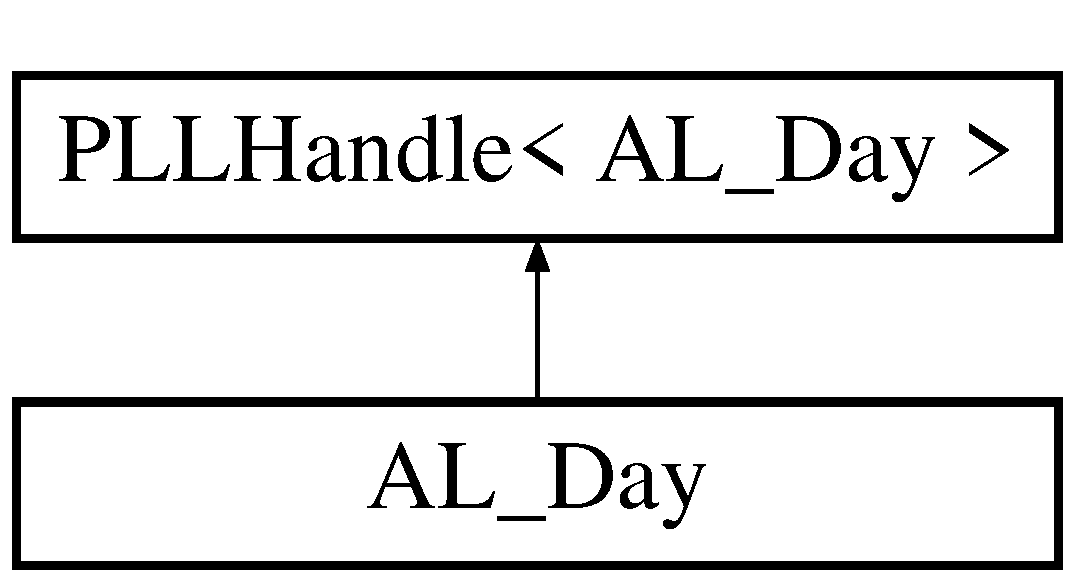
\includegraphics[height=2cm]{classAL__Day}
\end{center}
\end{figure}
\subsection*{Public Types}
\begin{CompactItemize}
\item 
enum {\bf TC\_\-add\_\-method} \{ {\bf TAIL\_\-REPLACE}, 
{\bf RANDOM}, 
{\bf BEFORE\_\-HEAD}
 \}
\end{CompactItemize}
\subsection*{Public Methods}
\begin{CompactItemize}
\item 
{\bf AL\_\-Day} (time\_\-t dd, int typ, time\_\-t tcsec, time\_\-t dsmin, time\_\-t dmaxt=SECONDSPERDAY)
\item 
{\bf $\sim$AL\_\-Day} ()
\item 
int {\bf Day\-Type} ()
\item 
time\_\-t {\bf Day\-Date} ()
\item 
time\_\-t {\bf Day\-Start} ()
\item 
time\_\-t {\bf Day\-Start\-Min} ()
\item 
time\_\-t {\bf Day\-Maxt} ()
\item 
bool {\bf Expanded} ()
\item 
long {\bf Avail} ()
\item 
long {\bf Total} ()
\item 
{\bf AL\_\-TC} $\ast$ {\bf TC\_\-Head} ()
\item 
{\bf AL\_\-TC} $\ast$ {\bf TC\_\-Tail} ()
\item 
{\bf AL\_\-TD} $\ast$ {\bf TD\_\-Head} ()
\item 
{\bf AL\_\-TD} $\ast$ {\bf TD\_\-Tail} ()
\item 
long {\bf set\_\-avail} (time\_\-t av)
\item 
long {\bf available\_\-before} (time\_\-t {\bf td})
\item 
int {\bf days\_\-to} (time\_\-t {\bf td})
\item 
void {\bf create\_\-TCs} (bool setvalues={\bf false})
\item 
void {\bf add\_\-TCs} (long tcs, {\bf TC\_\-add\_\-method} m, time\_\-t addborder=MAXTIME\_\-T)
\item 
long {\bf expand} (long expandn, time\_\-t {\bf td})
\item 
float {\bf set\_\-TC\_\-values} (long \&i\_\-start, long i\_\-limit)
\item 
float {\bf allocate\_\-with\_\-value} (float uval, {\bf DIL\_\-entry} $\ast$de)
\item 
{\bf AL\_\-TC} $\ast$ {\bf Get\_\-Avail\_\-TC} (unsigned long n)
\item 
{\bf AL\_\-TC} $\ast$ {\bf allocate} ({\bf DIL\_\-entry} $\ast$de)
\item 
AL\_\-Day $\ast$ {\bf Add\_\-Target\_\-Date} ({\bf DIL\_\-entry} $\ast$de)
\item 
long {\bf remove\_\-unused\_\-TCs} ()
\item 
float {\bf linear\_\-day\_\-distribution} (time\_\-t {\bf td})
\item 
float {\bf squared\_\-day\_\-distribution} (time\_\-t {\bf td})
\end{CompactItemize}
\subsection*{Public Attributes}
\begin{CompactItemize}
\item 
{\bf PLLRoot}$<$ {\bf AL\_\-TC} $>$ {\bf tc}
\item 
{\bf PLLRoot}$<$ {\bf AL\_\-TD} $>$ {\bf td}
\item 
float {\bf val}
\end{CompactItemize}
\subsection*{Protected Attributes}
\begin{CompactItemize}
\item 
int {\bf daytype}
\item 
long {\bf avail}
\item 
long {\bf tot}
\item 
time\_\-t {\bf daydate}
\item 
time\_\-t {\bf daystart}
\item 
time\_\-t {\bf daystartmin}
\item 
time\_\-t {\bf daymaxt}
\item 
time\_\-t {\bf tcseconds}
\item 
bool {\bf expanded}
\item 
long {\bf cache\_\-i\_\-start}
\item 
long {\bf cache\_\-i\_\-limit}
\end{CompactItemize}


\subsection{Member Enumeration Documentation}
\index{AL_Day@{AL\_\-Day}!TC_add_method@{TC\_\-add\_\-method}}
\index{TC_add_method@{TC\_\-add\_\-method}!AL_Day@{AL\_\-Day}}
\subsubsection{\setlength{\rightskip}{0pt plus 5cm}enum AL\_\-Day::TC\_\-add\_\-method}\label{classAL__Day_s3}


\begin{Desc}
\item[Enumeration values:]\par
\begin{description}
\index{TAIL_REPLACE@{TAIL\_\-REPLACE}!AL_Day@{AL\_\-Day}}\index{AL_Day@{AL\_\-Day}!TAIL_REPLACE@{TAIL\_\-REPLACE}}\item[{\em 
{\em TAIL\_\-REPLACE}\label{classAL__Day_s3s0}
}]\index{RANDOM@{RANDOM}!AL_Day@{AL\_\-Day}}\index{AL_Day@{AL\_\-Day}!RANDOM@{RANDOM}}\item[{\em 
{\em RANDOM}\label{classAL__Day_s3s1}
}]\index{BEFORE_HEAD@{BEFORE\_\-HEAD}!AL_Day@{AL\_\-Day}}\index{AL_Day@{AL\_\-Day}!BEFORE_HEAD@{BEFORE\_\-HEAD}}\item[{\em 
{\em BEFORE\_\-HEAD}\label{classAL__Day_s3s2}
}]\end{description}
\end{Desc}



Definition at line 887 of file dil2al.hh.

Referenced by expand().



\footnotesize\begin{verbatim}887 { TAIL_REPLACE, RANDOM, BEFORE_HEAD };
\end{verbatim}\normalsize 


\subsection{Constructor \& Destructor Documentation}
\index{AL_Day@{AL\_\-Day}!AL_Day@{AL\_\-Day}}
\index{AL_Day@{AL\_\-Day}!AL_Day@{AL\_\-Day}}
\subsubsection{\setlength{\rightskip}{0pt plus 5cm}AL\_\-Day::AL\_\-Day (time\_\-t {\em dd}, int {\em typ}, time\_\-t {\em tcsec}, time\_\-t {\em dsmin}, time\_\-t {\em dmaxt} = SECONDSPERDAY)}\label{classAL__Day_a0}




Definition at line 391 of file alcomp.cc.

References daystart, daystartmin, false, and SECONDSPERDAY.



\footnotesize\begin{verbatim}391                                                                                           :
392                 daystartmin(dsmin), daymaxt(dmaxt), daytype(typ), avail(0), tot(0), daydate(dd),
393                 tcseconds(tcsec), expanded(false), cache_i_start(0), cache_i_limit(0), val(0.0) {
394         if (alworkdaystart>=daystartmin) daystart = alworkdaystart;
395         else daystart = daystartmin;
396 }

\end{verbatim}\normalsize 
\index{AL_Day@{AL\_\-Day}!~AL_Day@{$\sim$AL\_\-Day}}
\index{~AL_Day@{$\sim$AL\_\-Day}!AL_Day@{AL\_\-Day}}
\subsubsection{\setlength{\rightskip}{0pt plus 5cm}AL\_\-Day::$\sim$AL\_\-Day ()\hspace{0.3cm}{\tt  [inline]}}\label{classAL__Day_a1}




Definition at line 864 of file dil2al.hh.



\footnotesize\begin{verbatim}864 {} 
\end{verbatim}\normalsize 


\subsection{Member Function Documentation}
\index{AL_Day@{AL\_\-Day}!Add_Target_Date@{Add\_\-Target\_\-Date}}
\index{Add_Target_Date@{Add\_\-Target\_\-Date}!AL_Day@{AL\_\-Day}}
\subsubsection{\setlength{\rightskip}{0pt plus 5cm}AL\_\-Day $\ast$ AL\_\-Day::Add\_\-Target\_\-Date ({\bf DIL\_\-entry} $\ast$ {\em de})}\label{classAL__Day_a24}




Definition at line 649 of file alcomp.cc.

References daydate, PLLRoot$<$ AL\_\-TD $>$::link\_\-before(), PLLHandle$<$ AL\_\-Day $>$::Next(), PLLHandle$<$ AL\_\-Day $>$::Prev(), SECONDSPERDAY, DIL\_\-entry::Target\_\-Date(), and td.

Referenced by Active\_\-List::Add\_\-Target\_\-Date().



\footnotesize\begin{verbatim}649                                                {
650 // Adds a target date reference to the day that contains it
651         if (!de) return NULL;
652         time_t tdiff = de->Target_Date() - daydate;
653         if (tdiff<0) {
654                 if (Prev()) return Prev()->Add_Target_Date(de);
655                 return NULL;
656         }
657         if (tdiff>=SECONDSPERDAY) {
658                 if (Next()) return Next()->Add_Target_Date(de);
659                 return NULL;
660         }
661         AL_TD * atd = new AL_TD(*de);
662         td.link_before(atd);
663         return this;
664 }
\end{verbatim}\normalsize 
\index{AL_Day@{AL\_\-Day}!add_TCs@{add\_\-TCs}}
\index{add_TCs@{add\_\-TCs}!AL_Day@{AL\_\-Day}}
\subsubsection{\setlength{\rightskip}{0pt plus 5cm}void AL\_\-Day::add\_\-TCs (long {\em tcs}, {\bf TC\_\-add\_\-method} {\em m}, time\_\-t {\em addborder} = MAXTIME\_\-T)}\label{classAL__Day_a18}




Definition at line 442 of file alcomp.cc.

References avail, BEFORE\_\-HEAD, expanded, PLLRoot$<$ AL\_\-TC $>$::head(), PLLRoot$<$ AL\_\-TC $>$::length(), PLLRoot$<$ AL\_\-TC $>$::link\_\-after(), PLLRoot$<$ AL\_\-TC $>$::link\_\-before(), MAXTIME\_\-T, RANDOM, AL\_\-TC::Set\_\-DE(), TAIL\_\-REPLACE, DIL\_\-entry::Target\_\-Date(), tc, and tot.

Referenced by expand().



\footnotesize\begin{verbatim}442                                                                             {
443 // safely add task chunks to a day
444 // links new task chunks if tchead!=NULL, using TAIL_REPLACE,
445 // RANDOM or BEFORE_HEAD methods, TAIL_REPLACE and RANDOM
446 // methods use the addborder parameter
447 // (see <A HREF="al-day-expand.fig">al-day-expand.fig</A>)
448 // uses tchead.length() to insure that tot will
449 // equal tchead.length() if tchead!=NULL
450         expanded = true;
451         avail += tcs;
452         tot += tcs;
453         if (tc.head()) {
454                 long linked = tc.length(), tci;
455                 tcs = tot - linked; // recalculated to insure at least tot TCs
456                 if (tcs<0) tcs = 0;
457                 switch (m) {
458                         case TAIL_REPLACE:
459                                 // Place empty TCs at tail and move de pointers at chosen
460                                 // random location to those TCs if de->Target_Date()>addborder
461                                 for (; tcs>0; tcs--) {
462                                         AL_TC * altc = new AL_TC();
463                                         tc.link_before(altc); linked++;
464                                         tci = (unsigned long) rint(((float) linked)*(((float) rand()) / ((float) RAND_MAX)));
465                                         if (tc[tci]) {
466                                                 DIL_entry * de = tc[tci]->Get_DE();
467                                                 if (de) if (de->Target_Date()>addborder) altc->Set_DE(tc[tci]->Set_DE(NULL));
468                                         }
469                                 }
470                                 break;
471                         case RANDOM:
472                                 // Place empty TCs at head and move de pointers at chosen
473                                 // random location to those TCs
474                                 if (linked>addborder) linked = (long) addborder; // number of TCs prior to tdiff
475                                 for (; tcs>0; tcs--) {
476                                         AL_TC * altc = new AL_TC();
477                                         tc.link_after(altc); linked++;
478                                         tci = (unsigned long) rint(((float) linked)*(((float) rand()) / ((float) RAND_MAX)));
479                                         if (tc[tci]) {
480                                                 DIL_entry * de = tc[tci]->Get_DE();
481                                                 if (de) altc->Set_DE(tc[tci]->Set_DE(NULL));
482                                         }
483                                 }
484                                 break;
485                         case BEFORE_HEAD:
486                                 // link tcs empty TCs before head
487                                 for (; tcs>0; tcs--) tc.link_after(new AL_TC());
488                                 break;
489                 }
490         }
491 }
\end{verbatim}\normalsize 
\index{AL_Day@{AL\_\-Day}!allocate@{allocate}}
\index{allocate@{allocate}!AL_Day@{AL\_\-Day}}
\subsubsection{\setlength{\rightskip}{0pt plus 5cm}{\bf AL\_\-TC} $\ast$ AL\_\-Day::allocate ({\bf DIL\_\-entry} $\ast$ {\em de})}\label{classAL__Day_a23}




Definition at line 628 of file alcomp.cc.

References AL\_\-TC::allocate(), Avail(), avail, create\_\-TCs(), Day\-Date(), PLLRoot$<$ AL\_\-TC $>$::head(), PLLHandle$<$ AL\_\-Day $>$::Next(), tc, time\_\-stamp(), Total(), and VOUT.

Referenced by Active\_\-List::allocate().



\footnotesize\begin{verbatim}628                                        {
629 // allocates de to the first available task
630 // chunk in this day or following days
631 // returns the allocated task chunk
632 // creates task chunks if necessary where tchead==NULL
633         if (avail<=0) {
634                 if (Next()) return Next()->allocate(de);
635                 return NULL;
636         }
637 #ifdef DETAILED_AL_DIAGNOSTIC_OUTPUT
638         VOUT << "A>" << time_stamp("%Y%m%d",DayDate()) << ": (" << Total() << ',' << Avail() << ')';
639 #endif
640         create_TCs();
641         AL_TC * atc = tc.head()->allocate(de);
642         if (atc) avail--;
643 #ifdef DETAILED_AL_DIAGNOSTIC_OUTPUT
644         VOUT << "->(" << Total() << ',' << Avail() << ")\n";
645 #endif
646         return atc;
647 }
\end{verbatim}\normalsize 
\index{AL_Day@{AL\_\-Day}!allocate_with_value@{allocate\_\-with\_\-value}}
\index{allocate_with_value@{allocate\_\-with\_\-value}!AL_Day@{AL\_\-Day}}
\subsubsection{\setlength{\rightskip}{0pt plus 5cm}float AL\_\-Day::allocate\_\-with\_\-value (float {\em uval}, {\bf DIL\_\-entry} $\ast$ {\em de})}\label{classAL__Day_a21}




Definition at line 593 of file alcomp.cc.

References AL\_\-TC::allocate\_\-with\_\-value(), avail, Avail(), create\_\-TCs(), Day\-Date(), PLLRoot$<$ AL\_\-TC $>$::head(), PLLHandle$<$ AL\_\-Day $>$::Next(), tc, time\_\-stamp(), Total(), val, and VOUT.

Referenced by Active\_\-List::allocate\_\-with\_\-value().



\footnotesize\begin{verbatim}593                                                             {
594 // allocate a DIL entry to a task chunk according to
595 // a random value
596 // returns the value of the allocated task chunk
597 // creates TCs if necessary
598         if (val<uval) {
599                 if (Next()) return Next()->allocate_with_value(uval-val,de);
600                 return 0.0; // (error) no more days, value was beyond sum
601         }
602 #ifdef DETAILED_AL_DIAGNOSTIC_OUTPUT
603         VOUT << "V>" << time_stamp("%Y%m%d",DayDate()) << ": (" << Total() << ',' << Avail() << ')';
604 #endif
605         create_TCs(true); // create TCs if necessary
606         float v = tc.head()->allocate_with_value(uval,de);
607         if (v>0.0) {
608                 val -= v;
609                 avail--;
610         }
611 #ifdef DETAILED_AL_DIAGNOSTIC_OUTPUT
612         VOUT << "->(" << Total() << ',' << Avail() << ")\n";
613 #endif
614         return v;
615 }
\end{verbatim}\normalsize 
\index{AL_Day@{AL\_\-Day}!Avail@{Avail}}
\index{Avail@{Avail}!AL_Day@{AL\_\-Day}}
\subsubsection{\setlength{\rightskip}{0pt plus 5cm}long AL\_\-Day::Avail ()\hspace{0.3cm}{\tt  [inline]}}\label{classAL__Day_a8}




Definition at line 877 of file dil2al.hh.

References avail.

Referenced by allocate(), allocate\_\-with\_\-value(), and expand().



\footnotesize\begin{verbatim}877 { return avail; }
\end{verbatim}\normalsize 
\index{AL_Day@{AL\_\-Day}!available_before@{available\_\-before}}
\index{available_before@{available\_\-before}!AL_Day@{AL\_\-Day}}
\subsubsection{\setlength{\rightskip}{0pt plus 5cm}long AL\_\-Day::available\_\-before (time\_\-t {\em td})}\label{classAL__Day_a15}




Definition at line 418 of file alcomp.cc.

References avail, AL\_\-TC::available\_\-before(), daydate, Day\-Date(), daystart, EOUT, PLLHandle$<$ AL\_\-Day $>$::Next(), TC\_\-Head(), tcseconds, and td.



\footnotesize\begin{verbatim}418                                        {
419 // returns the number of task chunks available for allocation
420 // prior to a target date td
421 // avail, daystart, tcseconds and Next()->DayDate() must contain valid values
422 // *** might be sped up by putting a for-loop into the
423 //     corresponding Active_List function
424         if (Next()) if (td>=Next()->DayDate()) return avail + Next()->available_before(td); // target date is within a following day
425         time_t tdiff = td - (daydate+daystart);
426         if (tdiff<=0) return 0; // target date is earlier than or at work start offset
427 #ifdef DIAGNOSTIC_OUTPUT
428         EOUT << "@tdiff=" << tdiff << ", tcseconds=" << tcseconds << ", tdiff/tcseconds=" << tdiff/tcseconds << '@';
429 #endif
430         long TCs_before = tdiff / tcseconds; // can't exceed target date
431         if (TC_Head()) return TC_Head()->available_before(TCs_before); // count available TCs before target date
432         return TCs_before;
433 }
\end{verbatim}\normalsize 
\index{AL_Day@{AL\_\-Day}!create_TCs@{create\_\-TCs}}
\index{create_TCs@{create\_\-TCs}!AL_Day@{AL\_\-Day}}
\subsubsection{\setlength{\rightskip}{0pt plus 5cm}void AL\_\-Day::create\_\-TCs (bool {\em setvalues} = {\bf false})}\label{classAL__Day_a17}




Definition at line 580 of file alcomp.cc.

References cache\_\-i\_\-limit, cache\_\-i\_\-start, PLLRoot$<$ AL\_\-TC $>$::head(), PLLRoot$<$ AL\_\-TC $>$::link\_\-before(), tc, and tot.

Referenced by allocate(), allocate\_\-with\_\-value(), and Get\_\-Avail\_\-TC().



\footnotesize\begin{verbatim}580                                               {
581 // creates TCs and sets values according to a random
582 // distribution if setvalues==true, in which case it
583 // requires valid cache_i_start and cache_i_limit values
584         if (tc.head()) return;
585         AL_TC * atc;
586         for (long i = 0; i<tot; i++) {
587                 if (setvalues) atc = new AL_TC(i+cache_i_start,cache_i_limit);
588                 else atc = new AL_TC();
589                 tc.link_before(atc);
590         }
591 }
\end{verbatim}\normalsize 
\index{AL_Day@{AL\_\-Day}!DayDate@{DayDate}}
\index{DayDate@{DayDate}!AL_Day@{AL\_\-Day}}
\subsubsection{\setlength{\rightskip}{0pt plus 5cm}time\_\-t AL\_\-Day::Day\-Date ()\hspace{0.3cm}{\tt  [inline]}}\label{classAL__Day_a3}




Definition at line 872 of file dil2al.hh.

References daydate.

Referenced by Active\_\-List::Add\_\-Day(), AL\_\-Day\_\-Marker(), allocate(), allocate\_\-with\_\-value(), available\_\-before(), days\_\-to(), expand(), and generate\_\-AL().



\footnotesize\begin{verbatim}872 { return daydate; }
\end{verbatim}\normalsize 
\index{AL_Day@{AL\_\-Day}!DayMaxt@{DayMaxt}}
\index{DayMaxt@{DayMaxt}!AL_Day@{AL\_\-Day}}
\subsubsection{\setlength{\rightskip}{0pt plus 5cm}time\_\-t AL\_\-Day::Day\-Maxt ()\hspace{0.3cm}{\tt  [inline]}}\label{classAL__Day_a6}




Definition at line 875 of file dil2al.hh.

References daymaxt.

Referenced by AL\_\-Day\_\-Marker(), and generate\_\-AL().



\footnotesize\begin{verbatim}875 { return daymaxt; }
\end{verbatim}\normalsize 
\index{AL_Day@{AL\_\-Day}!days_to@{days\_\-to}}
\index{days_to@{days\_\-to}!AL_Day@{AL\_\-Day}}
\subsubsection{\setlength{\rightskip}{0pt plus 5cm}int AL\_\-Day::days\_\-to (time\_\-t {\em td})}\label{classAL__Day_a16}




Definition at line 435 of file alcomp.cc.

References Day\-Date(), PLLHandle$<$ AL\_\-Day $>$::Next(), and td.

Referenced by linear\_\-day\_\-distribution(), and squared\_\-day\_\-distribution().



\footnotesize\begin{verbatim}435                              {
436 // returns the number of days to the target date, including
437 // the current day and the day containing the target date
438         if (Next()) if (td>Next()->DayDate()) return 1 + Next()->days_to(td);
439         return 1;
440 }
\end{verbatim}\normalsize 
\index{AL_Day@{AL\_\-Day}!DayStart@{DayStart}}
\index{DayStart@{DayStart}!AL_Day@{AL\_\-Day}}
\subsubsection{\setlength{\rightskip}{0pt plus 5cm}time\_\-t AL\_\-Day::Day\-Start ()\hspace{0.3cm}{\tt  [inline]}}\label{classAL__Day_a4}




Definition at line 873 of file dil2al.hh.

References daystart.

Referenced by AL\_\-Day\_\-Marker(), generate\_\-AL(), and Active\_\-List::Initialize\_\-AL\_\-Length().



\footnotesize\begin{verbatim}873 { return daystart; }
\end{verbatim}\normalsize 
\index{AL_Day@{AL\_\-Day}!DayStartMin@{DayStartMin}}
\index{DayStartMin@{DayStartMin}!AL_Day@{AL\_\-Day}}
\subsubsection{\setlength{\rightskip}{0pt plus 5cm}time\_\-t AL\_\-Day::Day\-Start\-Min ()\hspace{0.3cm}{\tt  [inline]}}\label{classAL__Day_a5}




Definition at line 874 of file dil2al.hh.

References daystartmin.

Referenced by AL\_\-Day\_\-Marker(), and Active\_\-List::Initialize\_\-AL\_\-Length().



\footnotesize\begin{verbatim}874 { return daystartmin; }
\end{verbatim}\normalsize 
\index{AL_Day@{AL\_\-Day}!DayType@{DayType}}
\index{DayType@{DayType}!AL_Day@{AL\_\-Day}}
\subsubsection{\setlength{\rightskip}{0pt plus 5cm}int AL\_\-Day::Day\-Type ()\hspace{0.3cm}{\tt  [inline]}}\label{classAL__Day_a2}




Definition at line 871 of file dil2al.hh.

References daytype.

Referenced by AL\_\-Day\_\-Marker().



\footnotesize\begin{verbatim}871 { return daytype; }
\end{verbatim}\normalsize 
\index{AL_Day@{AL\_\-Day}!expand@{expand}}
\index{expand@{expand}!AL_Day@{AL\_\-Day}}
\subsubsection{\setlength{\rightskip}{0pt plus 5cm}long AL\_\-Day::expand (long {\em expandn}, time\_\-t {\em td})}\label{classAL__Day_a19}




Definition at line 494 of file alcomp.cc.

References add\_\-TCs(), Avail(), BEFORE\_\-HEAD, Day\-Date(), daydate, daymaxt, daystart, daystartmin, EOUT, RANDOM, TAIL\_\-REPLACE, TC\_\-add\_\-method, tcseconds, td, time\_\-stamp(), tot, Total(), and VOUT.

Referenced by Active\_\-List::expand().



\footnotesize\begin{verbatim}494                                            {
495 // expand work time by adding task chunks prior to
496 // the target date td
497 // returns the number of task chunks added (-1==error)
498 // (see <A HREF="al-day-expand.fig">al-day-expand.fig</A>)
499         if (expandn<=0) return 0;
500         const time_t tdiff(td - daydate); // target date limit (offset in current day)
501         // case: TD1 in al-day-expand.fig
502         if (tdiff<(daystartmin+tcseconds)) return 0;
503 #ifdef DETAILED_AL_DIAGNOSTIC_OUTPUT
504         VOUT << "E>" << time_stamp("%Y%m%d",DayDate()) << ": (" << Total() << ',' << Avail() << "), expand request = " << expandn << '\n';
505 #endif
506         long addabove = 0;
507         time_t dayend = daystart+(tot*tcseconds); // if tot==0 dayend is current time
508         // cases: TD4, TD5 and TD6 in al-day-expand.fig
509         if (tdiff>=(dayend+tcseconds)) { // TD beyond current end of day tasks
510                 time_t dayendmax = tdiff;
511                 if (tdiff>daymaxt) dayendmax = daymaxt; // day upper limit
512                 addabove = (dayendmax-dayend)/tcseconds; // count TCs that can be added prior to target date and daymaxt
513                 if (addabove>0) {
514                         if (addabove>expandn) addabove = expandn; // add expandn or fewer TCs above current dayend
515 #ifdef DETAILED_AL_DIAGNOSTIC_OUTPUT
516                         VOUT << "Ea>" << time_stamp("%Y%m%d",DayDate()) << ": (" << Total() << ',' << Avail() << ')';
517 #endif
518                         add_TCs(addabove,TAIL_REPLACE,daydate+dayendmax); // add empty TCs by replacing allocated TCs with target dates greater than dayendmax and moving those to the tail and update tot and avail
519                         expandn -= addabove;
520 #ifdef DETAILED_AL_DIAGNOSTIC_OUTPUT
521                         VOUT << "->(" << Total() << ',' << Avail() << ")\n";
522 #endif
523                         if (expandn<0) EOUT << "dil2al: Warning - Expansion exceeded requirement in AL_Day::expand()\n";
524                         if (expandn<=0) return addabove;
525                 }
526         }
527         // case: TD3 in al-day-expand.fig
528         time_t tlowerexpand = daystart;
529         TC_add_method m = RANDOM;
530         long totbeforetdiff = (tdiff-daystart)/tcseconds;
531         // case: TD2 in al-day-expand.fig
532         if (totbeforetdiff<=0) {
533                 tlowerexpand = tdiff;
534                 m = BEFORE_HEAD;
535         }
536         if (totbeforetdiff>tot) totbeforetdiff = tot;
537         time_t newdaystart = tlowerexpand - (expandn*tcseconds); // attempt to add expandn TCs prior to daystart
538         if (newdaystart<daystartmin) newdaystart = daystartmin; // daystart limit
539         long addbelow = (tlowerexpand-newdaystart)/tcseconds; // count TCs to be added prior to daystart
540         if (addbelow>0) { // add expandn or fewer TCs below min(daystart,TDtime)
541                 daystart = newdaystart;
542 #ifdef DETAILED_AL_DIAGNOSTIC_OUTPUT
543                 VOUT << "Eab>" << time_stamp("%Y%m%d",DayDate()) << ": (" << Total() << ',' << Avail() << ')';
544 #endif
545                 add_TCs(addbelow,m,totbeforetdiff); // add empty TCs before target date and update tot and avail
546 #ifdef DETAILED_AL_DIAGNOSTIC_OUTPUT
547                 VOUT << "->(" << Total() << ',' << Avail() << ")\n";
548 #endif
549                 return addabove+addbelow;
550         }
551 #ifdef DETAILED_AL_DIAGNOSTIC_OUTPUT
552         VOUT << "Ex>" << time_stamp("%Y%m%d",DayDate()) << ": (" << Total() << ',' << Avail() << ")\n";
553 #endif
554         return addabove;
555 }
\end{verbatim}\normalsize 
\index{AL_Day@{AL\_\-Day}!Expanded@{Expanded}}
\index{Expanded@{Expanded}!AL_Day@{AL\_\-Day}}
\subsubsection{\setlength{\rightskip}{0pt plus 5cm}bool AL\_\-Day::Expanded ()\hspace{0.3cm}{\tt  [inline]}}\label{classAL__Day_a7}




Definition at line 876 of file dil2al.hh.

References expanded.

Referenced by AL\_\-Day\_\-Marker().



\footnotesize\begin{verbatim}876 { return expanded; }
\end{verbatim}\normalsize 
\index{AL_Day@{AL\_\-Day}!Get_Avail_TC@{Get\_\-Avail\_\-TC}}
\index{Get_Avail_TC@{Get\_\-Avail\_\-TC}!AL_Day@{AL\_\-Day}}
\subsubsection{\setlength{\rightskip}{0pt plus 5cm}{\bf AL\_\-TC} $\ast$ AL\_\-Day::Get\_\-Avail\_\-TC (unsigned long {\em n})}\label{classAL__Day_a22}




Definition at line 617 of file alcomp.cc.

References avail, AL\_\-TC::avail\_\-el(), create\_\-TCs(), PLLRoot$<$ AL\_\-TC $>$::head(), PLLHandle$<$ AL\_\-Day $>$::Next(), and tc.

Referenced by Active\_\-List::Get\_\-Avail\_\-TC().



\footnotesize\begin{verbatim}617                                             {
618 // returns the nth available task chunk in the AL
619 // creates task chunks if necessary where tchead==NULL
620         if (avail<=n) {
621                 if (Next()) return Next()->Get_Avail_TC(n-avail);
622                 return NULL;
623         }
624         create_TCs();
625         return tc.head()->avail_el(n);
626 }
\end{verbatim}\normalsize 
\index{AL_Day@{AL\_\-Day}!linear_day_distribution@{linear\_\-day\_\-distribution}}
\index{linear_day_distribution@{linear\_\-day\_\-distribution}!AL_Day@{AL\_\-Day}}
\subsubsection{\setlength{\rightskip}{0pt plus 5cm}float AL\_\-Day::linear\_\-day\_\-distribution (time\_\-t {\em td})}\label{classAL__Day_a26}




Definition at line 702 of file alcomp.cc.

References days\_\-to(), PLL\_\-LOOP\_\-FORWARD, and td.

Referenced by Active\_\-List::expand().



\footnotesize\begin{verbatim}702                                                {
703 // linearly distribute values up to target date
704         float sumval = 0;
705         int tddays = days_to(td);
706         float fdays = (float) tddays;
707         long i = 0;
708         PLL_LOOP_FORWARD(AL_Day,this,(e->DayDate()<td)) {
709                 e->val = 1.0 - (aldaydistslope*((float) i/fdays));
710                 sumval += e->val;
711                 i++;
712         }
713         return sumval;
714 }
\end{verbatim}\normalsize 
\index{AL_Day@{AL\_\-Day}!remove_unused_TCs@{remove\_\-unused\_\-TCs}}
\index{remove_unused_TCs@{remove\_\-unused\_\-TCs}!AL_Day@{AL\_\-Day}}
\subsubsection{\setlength{\rightskip}{0pt plus 5cm}long AL\_\-Day::remove\_\-unused\_\-TCs ()}\label{classAL__Day_a25}




Definition at line 666 of file alcomp.cc.

References avail, AL\_\-TC::Get\_\-DE(), PLLRoot$<$ AL\_\-TC $>$::head(), PLLHandle$<$ AL\_\-TC $>$::Next(), PLLHandle$<$ AL\_\-Day $>$::Next(), PLLHandle$<$ AL\_\-TC $>$::remove(), tc, and tot.

Referenced by Active\_\-List::remove\_\-unused\_\-TCs().



\footnotesize\begin{verbatim}666                                {
667 // clean up by removing unused TCs
668 // returns remaining number of TCs in AL
669         if (!tc.head()) { // no TCs created in this day
670                 tot = 0;
671                 avail = 0;
672                 if (Next()) return Next()->remove_unused_TCs();
673                 return 0;
674         }
675         AL_TC * rtc, * atc = tc.head();
676         tot = 0; // insure correct count
677         while (atc) { // remove unused TCs in this day
678                 rtc = atc;
679                 atc = atc->Next();
680                 if (!rtc->Get_DE()) rtc->remove();
681                 else tot++; // faster than calling tchead->length()
682         }
683         avail = 0;
684         if (Next()) return tot + Next()->remove_unused_TCs();
685         return tot;
686 }
\end{verbatim}\normalsize 
\index{AL_Day@{AL\_\-Day}!set_avail@{set\_\-avail}}
\index{set_avail@{set\_\-avail}!AL_Day@{AL\_\-Day}}
\subsubsection{\setlength{\rightskip}{0pt plus 5cm}long AL\_\-Day::set\_\-avail (time\_\-t {\em av})}\label{classAL__Day_a14}




Definition at line 398 of file alcomp.cc.

References avail, daymaxt, daystartmin, EOUT, tcseconds, and tot.

Referenced by Active\_\-List::Initialize\_\-AL\_\-Length().



\footnotesize\begin{verbatim}398                                 {
399 // attempt to make av seconds available through task chunks
400 // returns the number of task chunks made available
401 // the number of task chunks is limited by (daymaxt-daystartmin)
402 // if av<0 no task chunks will be made available
403         time_t dtmax = daymaxt - daystartmin;
404 #ifdef DIAGNOSTIC_OUTPUT
405         EOUT << "dil2al: (DIAGNOSTICS) av = " << av << ", daymaxt = " << daymaxt << ", daystartmin = " << daystartmin << ", dtmax = " << dtmax << '\n';
406 #endif
407         if (av>0) {
408                 if (av>dtmax) av = dtmax;
409                 avail = av/tcseconds; // floor, can't exceed limit
410         } else avail = 0;
411         tot = avail; // initialized with all TCs available
412 #ifdef DIAGNOSTIC_OUTPUT
413         EOUT << "dil2al: (DIAGNOSTICS) av = " << av << ", avail = " << avail << ", tot = " << tot << '\n';
414 #endif
415         return avail;
416 }
\end{verbatim}\normalsize 
\index{AL_Day@{AL\_\-Day}!set_TC_values@{set\_\-TC\_\-values}}
\index{set_TC_values@{set\_\-TC\_\-values}!AL_Day@{AL\_\-Day}}
\subsubsection{\setlength{\rightskip}{0pt plus 5cm}float AL\_\-Day::set\_\-TC\_\-values (long \& {\em i\_\-start}, long {\em i\_\-limit})}\label{classAL__Day_a20}




Definition at line 557 of file alcomp.cc.

References avail, AL\_\-TC::avail\_\-el(), cache\_\-i\_\-limit, cache\_\-i\_\-start, daydate, EOUT, PLLRoot$<$ AL\_\-TC $>$::head(), linear\_\-distribution(), AL\_\-TC::set\_\-val(), tc, time\_\-stamp(), and val.



\footnotesize\begin{verbatim}557                                                         {
558 // set TC values within this day
559 // returns sum of TC values
560         float v;
561         cache_i_start = i_start;
562         cache_i_limit = i_limit;
563         val = 0.0;
564         for (long i=0; i<avail; i++) {
565                 if ((i+i_start)>=i_limit) v = 0.0;
566                 else v = linear_distribution((float) (i+i_start), (float) i_limit);
567                 if (tc.head()) {
568                         AL_TC * atc = tc.head()->avail_el(i);
569                         if (atc) atc->set_val(v);
570                         else EOUT << "dil2al: Available TC #" << i << " on day " << time_stamp("%Y%m%d",daydate) << " not found in AL_Day::set_TC_values(), continuing\n";
571                 }
572                 // assignment of values to remaining TCs occurs when
573                 // those TCs are created as a search enters them
574                 val += v; // store summed values of TCs for that day
575         }
576         i_start += avail;
577         return val;
578 }
\end{verbatim}\normalsize 
\index{AL_Day@{AL\_\-Day}!squared_day_distribution@{squared\_\-day\_\-distribution}}
\index{squared_day_distribution@{squared\_\-day\_\-distribution}!AL_Day@{AL\_\-Day}}
\subsubsection{\setlength{\rightskip}{0pt plus 5cm}float AL\_\-Day::squared\_\-day\_\-distribution (time\_\-t {\em td})}\label{classAL__Day_a27}




Definition at line 688 of file alcomp.cc.

References days\_\-to(), PLL\_\-LOOP\_\-FORWARD, and td.

Referenced by Active\_\-List::expand().



\footnotesize\begin{verbatim}688                                                 {
689 // distribute values up to target date according to a squared function
690         float sumval = 0;
691         int tddays = days_to(td);
692         float fdays = (float) tddays, fi = 0.0;
693         long i = 0;
694         PLL_LOOP_FORWARD(AL_Day,this,(e->DayDate()<td)) {
695                 e->val = 1.0 - (aldaydistslope*(fi*fi));
696                 sumval += e->val;
697                 i++; fi = ((float) i)/fdays;
698         }
699         return sumval;
700 }
\end{verbatim}\normalsize 
\index{AL_Day@{AL\_\-Day}!TC_Head@{TC\_\-Head}}
\index{TC_Head@{TC\_\-Head}!AL_Day@{AL\_\-Day}}
\subsubsection{\setlength{\rightskip}{0pt plus 5cm}{\bf AL\_\-TC}$\ast$ AL\_\-Day::TC\_\-Head ()\hspace{0.3cm}{\tt  [inline]}}\label{classAL__Day_a10}




Definition at line 879 of file dil2al.hh.

References PLLRoot$<$ PLLType $>$::head().

Referenced by available\_\-before().



\footnotesize\begin{verbatim}879 { return tc.head(); }
\end{verbatim}\normalsize 
\index{AL_Day@{AL\_\-Day}!TC_Tail@{TC\_\-Tail}}
\index{TC_Tail@{TC\_\-Tail}!AL_Day@{AL\_\-Day}}
\subsubsection{\setlength{\rightskip}{0pt plus 5cm}{\bf AL\_\-TC}$\ast$ AL\_\-Day::TC\_\-Tail ()\hspace{0.3cm}{\tt  [inline]}}\label{classAL__Day_a11}




Definition at line 880 of file dil2al.hh.

References PLLRoot$<$ PLLType $>$::tail().



\footnotesize\begin{verbatim}880 { return tc.tail(); }
\end{verbatim}\normalsize 
\index{AL_Day@{AL\_\-Day}!TD_Head@{TD\_\-Head}}
\index{TD_Head@{TD\_\-Head}!AL_Day@{AL\_\-Day}}
\subsubsection{\setlength{\rightskip}{0pt plus 5cm}{\bf AL\_\-TD}$\ast$ AL\_\-Day::TD\_\-Head ()\hspace{0.3cm}{\tt  [inline]}}\label{classAL__Day_a12}




Definition at line 881 of file dil2al.hh.

References PLLRoot$<$ PLLType $>$::head().

Referenced by AL\_\-Day\_\-Marker().



\footnotesize\begin{verbatim}881 { return td.head(); }
\end{verbatim}\normalsize 
\index{AL_Day@{AL\_\-Day}!TD_Tail@{TD\_\-Tail}}
\index{TD_Tail@{TD\_\-Tail}!AL_Day@{AL\_\-Day}}
\subsubsection{\setlength{\rightskip}{0pt plus 5cm}{\bf AL\_\-TD}$\ast$ AL\_\-Day::TD\_\-Tail ()\hspace{0.3cm}{\tt  [inline]}}\label{classAL__Day_a13}




Definition at line 882 of file dil2al.hh.

References PLLRoot$<$ PLLType $>$::tail().



\footnotesize\begin{verbatim}882 { return td.tail(); }
\end{verbatim}\normalsize 
\index{AL_Day@{AL\_\-Day}!Total@{Total}}
\index{Total@{Total}!AL_Day@{AL\_\-Day}}
\subsubsection{\setlength{\rightskip}{0pt plus 5cm}long AL\_\-Day::Total ()\hspace{0.3cm}{\tt  [inline]}}\label{classAL__Day_a9}




Definition at line 878 of file dil2al.hh.

References tot.

Referenced by AL\_\-Day\_\-Marker(), allocate(), allocate\_\-with\_\-value(), and expand().



\footnotesize\begin{verbatim}878 { return tot; }
\end{verbatim}\normalsize 


\subsection{Member Data Documentation}
\index{AL_Day@{AL\_\-Day}!avail@{avail}}
\index{avail@{avail}!AL_Day@{AL\_\-Day}}
\subsubsection{\setlength{\rightskip}{0pt plus 5cm}long AL\_\-Day::avail\hspace{0.3cm}{\tt  [protected]}}\label{classAL__Day_n1}




Definition at line 850 of file dil2al.hh.

Referenced by add\_\-TCs(), allocate(), allocate\_\-with\_\-value(), Avail(), available\_\-before(), Get\_\-Avail\_\-TC(), remove\_\-unused\_\-TCs(), set\_\-avail(), and set\_\-TC\_\-values().\index{AL_Day@{AL\_\-Day}!cache_i_limit@{cache\_\-i\_\-limit}}
\index{cache_i_limit@{cache\_\-i\_\-limit}!AL_Day@{AL\_\-Day}}
\subsubsection{\setlength{\rightskip}{0pt plus 5cm}long AL\_\-Day::cache\_\-i\_\-limit\hspace{0.3cm}{\tt  [protected]}}\label{classAL__Day_n10}




Definition at line 859 of file dil2al.hh.

Referenced by create\_\-TCs(), and set\_\-TC\_\-values().\index{AL_Day@{AL\_\-Day}!cache_i_start@{cache\_\-i\_\-start}}
\index{cache_i_start@{cache\_\-i\_\-start}!AL_Day@{AL\_\-Day}}
\subsubsection{\setlength{\rightskip}{0pt plus 5cm}long AL\_\-Day::cache\_\-i\_\-start\hspace{0.3cm}{\tt  [protected]}}\label{classAL__Day_n9}




Definition at line 858 of file dil2al.hh.

Referenced by create\_\-TCs(), and set\_\-TC\_\-values().\index{AL_Day@{AL\_\-Day}!daydate@{daydate}}
\index{daydate@{daydate}!AL_Day@{AL\_\-Day}}
\subsubsection{\setlength{\rightskip}{0pt plus 5cm}time\_\-t AL\_\-Day::daydate\hspace{0.3cm}{\tt  [protected]}}\label{classAL__Day_n3}




Definition at line 852 of file dil2al.hh.

Referenced by Add\_\-Target\_\-Date(), available\_\-before(), Day\-Date(), expand(), and set\_\-TC\_\-values().\index{AL_Day@{AL\_\-Day}!daymaxt@{daymaxt}}
\index{daymaxt@{daymaxt}!AL_Day@{AL\_\-Day}}
\subsubsection{\setlength{\rightskip}{0pt plus 5cm}time\_\-t AL\_\-Day::daymaxt\hspace{0.3cm}{\tt  [protected]}}\label{classAL__Day_n6}




Definition at line 855 of file dil2al.hh.

Referenced by Day\-Maxt(), expand(), and set\_\-avail().\index{AL_Day@{AL\_\-Day}!daystart@{daystart}}
\index{daystart@{daystart}!AL_Day@{AL\_\-Day}}
\subsubsection{\setlength{\rightskip}{0pt plus 5cm}time\_\-t AL\_\-Day::daystart\hspace{0.3cm}{\tt  [protected]}}\label{classAL__Day_n4}




Definition at line 853 of file dil2al.hh.

Referenced by AL\_\-Day(), available\_\-before(), Day\-Start(), and expand().\index{AL_Day@{AL\_\-Day}!daystartmin@{daystartmin}}
\index{daystartmin@{daystartmin}!AL_Day@{AL\_\-Day}}
\subsubsection{\setlength{\rightskip}{0pt plus 5cm}time\_\-t AL\_\-Day::daystartmin\hspace{0.3cm}{\tt  [protected]}}\label{classAL__Day_n5}




Definition at line 854 of file dil2al.hh.

Referenced by AL\_\-Day(), Day\-Start\-Min(), expand(), and set\_\-avail().\index{AL_Day@{AL\_\-Day}!daytype@{daytype}}
\index{daytype@{daytype}!AL_Day@{AL\_\-Day}}
\subsubsection{\setlength{\rightskip}{0pt plus 5cm}int AL\_\-Day::daytype\hspace{0.3cm}{\tt  [protected]}}\label{classAL__Day_n0}




Definition at line 849 of file dil2al.hh.

Referenced by Day\-Type().\index{AL_Day@{AL\_\-Day}!expanded@{expanded}}
\index{expanded@{expanded}!AL_Day@{AL\_\-Day}}
\subsubsection{\setlength{\rightskip}{0pt plus 5cm}bool AL\_\-Day::expanded\hspace{0.3cm}{\tt  [protected]}}\label{classAL__Day_n8}




Definition at line 857 of file dil2al.hh.

Referenced by add\_\-TCs(), and Expanded().\index{AL_Day@{AL\_\-Day}!tc@{tc}}
\index{tc@{tc}!AL_Day@{AL\_\-Day}}
\subsubsection{\setlength{\rightskip}{0pt plus 5cm}{\bf PLLRoot}$<${\bf AL\_\-TC}$>$ AL\_\-Day::tc}\label{classAL__Day_m0}




Definition at line 866 of file dil2al.hh.

Referenced by add\_\-TCs(), allocate(), allocate\_\-with\_\-value(), create\_\-TCs(), Get\_\-Avail\_\-TC(), remove\_\-unused\_\-TCs(), and set\_\-TC\_\-values().\index{AL_Day@{AL\_\-Day}!tcseconds@{tcseconds}}
\index{tcseconds@{tcseconds}!AL_Day@{AL\_\-Day}}
\subsubsection{\setlength{\rightskip}{0pt plus 5cm}time\_\-t AL\_\-Day::tcseconds\hspace{0.3cm}{\tt  [protected]}}\label{classAL__Day_n7}




Definition at line 856 of file dil2al.hh.

Referenced by available\_\-before(), expand(), and set\_\-avail().\index{AL_Day@{AL\_\-Day}!td@{td}}
\index{td@{td}!AL_Day@{AL\_\-Day}}
\subsubsection{\setlength{\rightskip}{0pt plus 5cm}{\bf PLLRoot}$<${\bf AL\_\-TD}$>$ AL\_\-Day::td}\label{classAL__Day_m1}




Definition at line 867 of file dil2al.hh.

Referenced by Add\_\-Target\_\-Date(), available\_\-before(), days\_\-to(), expand(), linear\_\-day\_\-distribution(), and squared\_\-day\_\-distribution().\index{AL_Day@{AL\_\-Day}!tot@{tot}}
\index{tot@{tot}!AL_Day@{AL\_\-Day}}
\subsubsection{\setlength{\rightskip}{0pt plus 5cm}long AL\_\-Day::tot\hspace{0.3cm}{\tt  [protected]}}\label{classAL__Day_n2}




Definition at line 851 of file dil2al.hh.

Referenced by add\_\-TCs(), create\_\-TCs(), expand(), remove\_\-unused\_\-TCs(), set\_\-avail(), and Total().\index{AL_Day@{AL\_\-Day}!val@{val}}
\index{val@{val}!AL_Day@{AL\_\-Day}}
\subsubsection{\setlength{\rightskip}{0pt plus 5cm}float AL\_\-Day::val}\label{classAL__Day_m2}




Definition at line 869 of file dil2al.hh.

Referenced by allocate\_\-with\_\-value(), Active\_\-List::expand(), and set\_\-TC\_\-values().

The documentation for this class was generated from the following files:\begin{CompactItemize}
\item 
{\bf dil2al.hh}\item 
{\bf alcomp.cc}\end{CompactItemize}
